\documentclass{article}
\usepackage[backend=biber,citestyle=ieee]{biblatex}

\usepackage[english]{babel}
% \usepackage[swedish]{babel}

\usepackage{graphicx}
\usepackage{csquotes}
\usepackage{float}
\usepackage{datetime}
\usepackage[title]{appendix}


% \usepackage{a4wide} 

\usepackage{fancyhdr}   %page header
\pagestyle{fancy}

\usepackage{xcolor}
\usepackage{listings}

\definecolor{codegreen}{rgb}{0,0.6,0}
\definecolor{codegray}{rgb}{0.5,0.5,0.5}
\definecolor{codepurple}{rgb}{0.58,0,0.82}
\definecolor{backcolour}{rgb}{0.95,0.95,0.95}
\lstdefinestyle{mystyle}{
    backgroundcolor=\color{backcolour},   
    commentstyle=\color{codegreen},
    keywordstyle=\color{magenta},
    numberstyle=\tiny\color{codegray},
    stringstyle=\color{codepurple},
    basicstyle=\ttfamily\footnotesize,
    breakatwhitespace=false,         
    breaklines=true,                 
    captionpos=b,                    
    keepspaces=false,                 
    numbers=left,                    
    numbersep=5pt,                  
    showspaces=false,                
    showstringspaces=false,
    showtabs=false,                  
    tabsize=1
}
\lstset{style=mystyle}

\addbibresource{sources.bib}

\newcommand{\getauthor}{Oscar Fredriksson} %Author
\newcommand{\gettitle}{Title goes here} %Title

\newdateformat{daymonthyear}{\ordinal{DAY} \monthname[\THEMONTH] \THEYEAR} %Date

\title{\gettitle}
\author{\getauthor}

\date{\daymonthyear\today} %Remove for swedish date

\begin{document}

    % Title 
    \pagenumbering{gobble}
    \maketitle
    \newpage

    % Page header and footer
    \pagenumbering{arabic}
    \fancyhf{}
    \lhead{\getauthor}
    \rhead{\gettitle}
    \rfoot \thepage

    % Document starts here
    \section{Visualization using Contour}
    The values from lab 1 was tweaked slightly to achieve a similar 

    \begin{figure}[H]
        \centering
        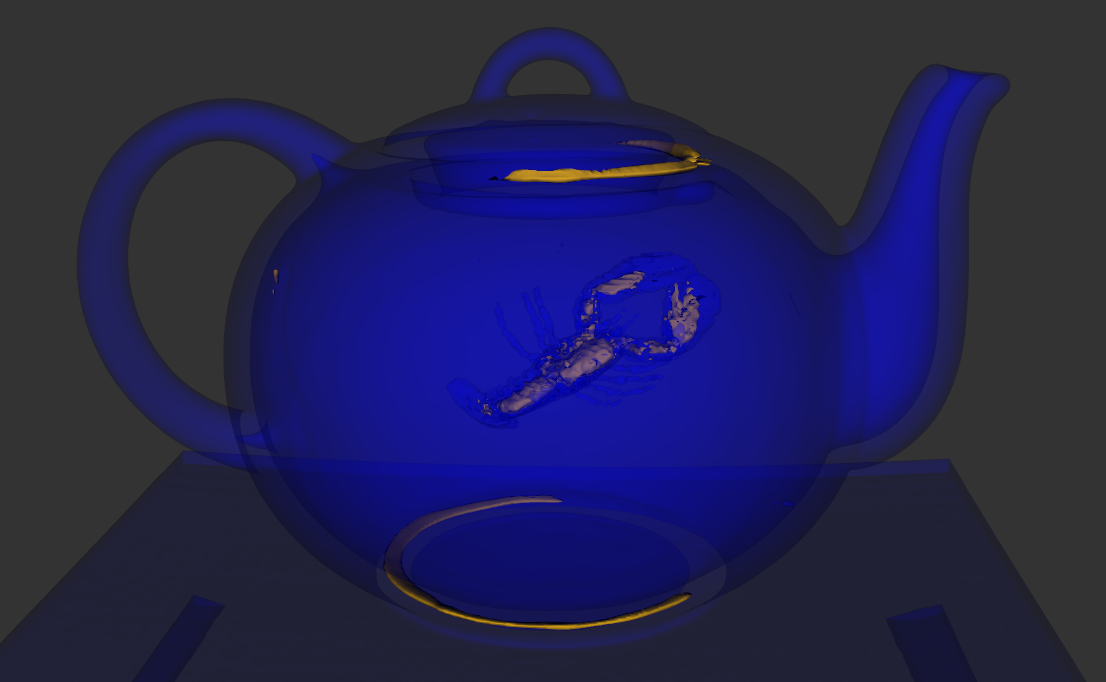
\includegraphics[width=0.75\textwidth]{../img/contour.png}
        \caption{The  teapot  visualized  using  contour  with  values  30  (blue)  and  130(yellow) along with an opacity value of 0.2 to see the lobster inside.}
        \label{fig:contour}
    \end{figure}

    \section{Visualization using Clip}
    The values from lab 1 was tweaked slightly to achieve a similar 

    \begin{figure}[H]
        \centering
        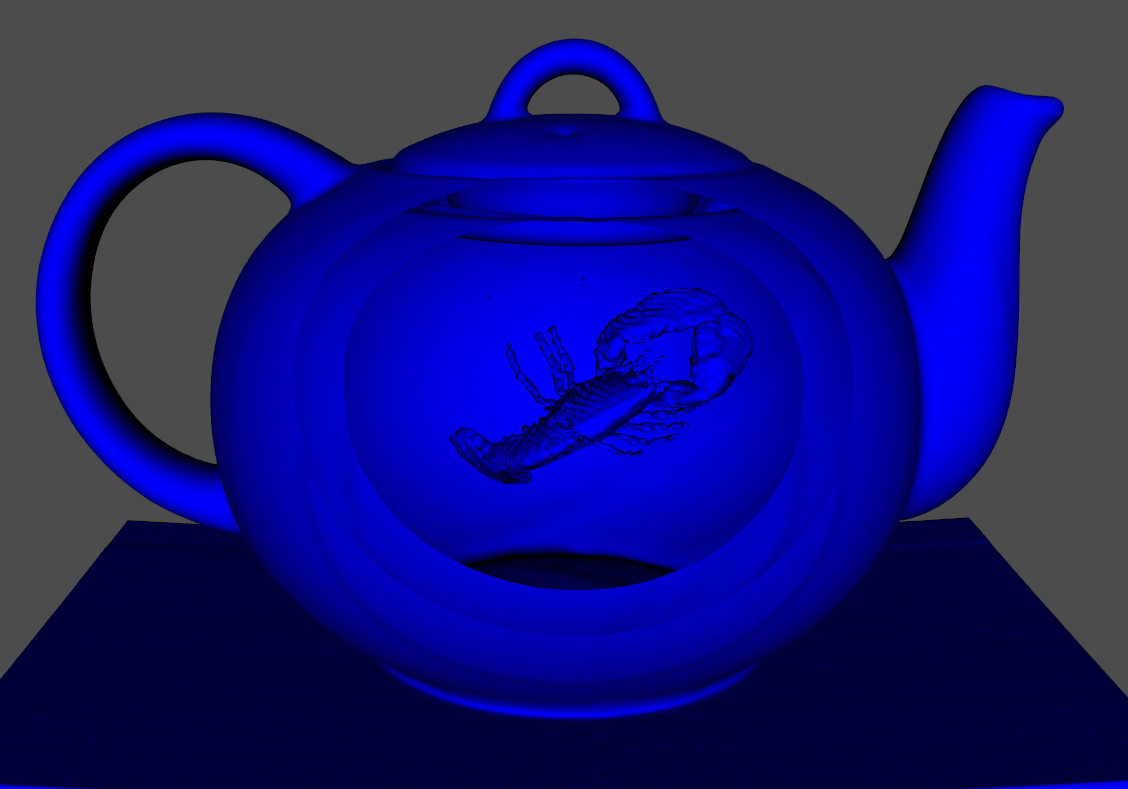
\includegraphics[width=0.75\textwidth]{../img/clip.png}
        \caption{}
        \label{fig:clip}
    \end{figure}



    % Sources
    % \newpage
    % \printbibliography

    % Appendices
    \newpage
    \begin{appendices}

        \section{Contour visualization code}
        \label{appendix:contour}

        \lstinputlisting[language=python]{../src/contour.py}

        \section{Contour visualization code}
        \label{appendix:clip}

        \lstinputlisting[language=python]{../src/clip.py}

    \end{appendices}

\end{document}

% Centered figure with caption:
% \begin{figure}[H]
%     \centering
%     \includegraphics[width=1\textwidth]{%path} 
%     \caption{}
%     \label{fig:}
% \end{figure}

% Side by side figures:
% \begin{figure}[H]
%     \centering
%     \subfloat{{\includegraphics[width=0.46\textwidth]{%path} }}%
%     \qquad
%     \subfloat{{\includegraphics[width=0.46\textwidth]{%path} }}%
%     \caption{}
%     \label{fig:}
% \end{figure}

% Table with caption:
% \begin{table}[H]      
%     \begin{center}
%     \begin{tabular}{|c|c|} 
%         \hline
%         \textbf{} & \textbf{} \\\hline\hline
%          &  \\\hline 
%     \end{tabular}
%     \end{center}
%     \caption{}
%     \label{tab:}
% \end{table}